%************************************************
\chapter{Distance, Probability Spaces and Information Theory}\label{ch:distance_probability_spaces_and_information_theory}
%************************************************
%\begin{flushleft}{\slshape    
%    At the time, Nixon was normalizing relations with China.  
%    I figured that if he could normalize relations, then so could I} \\ \medskip
%    --- Edgar Codd
%\end{flushleft}
%
In this chapter we review the basics of information theory starting with a brief recap of probability, then introduce information, and finally derive entropy as defined by Shannon in his seminal work\cite{Shannon:1948} to serve as a foundation for later chapters.

\section{Distance}

% ********************* %
\subsection{Metric spaces}
% ********************* %
A metric space is simply a set of objects which have distances between them. Our own understanding of the physical world informs our intuition for the postulates of a metric -- there cannot be a negative distance; the distance between points is the same in both directions; if there is no distance between two objects they must be be at the same point (be the same object) -- likewise, there is no distance between two identical objects; and finally, there is no shorter distance between two objects by taking a detour through a third object.

These axioms are defined formally as follows:
%
\begin{mydef} 
A metric space $M$ is an ordered pair $(X,d)$ where $X$ is a set and $d: X \times X \rightarrow \mathbb{R}$ is a metric that defines the distance between elements in $X$. Furthermore, $d$ must satisfy the following properties:
 \begin{flalign*}
  &\quad \forall x,y \in X, 
  && d(x, y) \geq 0    \tag{positiveness}&\qquad &\\
  %
  &\quad\forall x,y \in X, 
  && d(x, y) = d(y, x) \tag{symmetry}&&\\
  %
  &\quad\forall x,y \in X, 
  && d(x, y) = 0  \Leftrightarrow  x = y \tag{reflexitivity}&&\\
  %
  &\quad\forall x,y,z \in X, 
  && d(x, z)  \leq d(x, y) + d(y, z) \tag{triangle inequality}&&
 \end{flalign*} 
\end{mydef}
% 
% ********************* %
\subsection{Vector spaces}
% ********************* %
Vector spaces are more specific than metric spaces, since they allow the elements of the space to be added or scaled to produce new elements.%\ToDo{Give more motivation for describing this}
\begin{mydef} 
A metric space $M = (V, d)$ is also a vector space if $V$ is closed under addition and multiplication operations.
%
Furthermore, the following axioms must hold for addition:
%
 \begin{flalign*}
  &\quad \forall \mathbf{x},\mathbf{y} \in V,  
  && \mathbf{x} + \mathbf{y} =  \mathbf{y} + \mathbf{x}  \tag{commutativity}&\qquad\qquad&\\
  %
  &\quad \forall \mathbf{x},\mathbf{y},\mathbf{z} \in V, 
  && (\mathbf{x}+\mathbf{y})+\mathbf{z}  = \mathbf{x}+(\mathbf{y}+\mathbf{z})  \tag{associativity}&&\\
  %
  &\quad \forall \mathbf{x} \in V, 
  && \mathbf{0} + \mathbf{x} = \mathbf{x}  \tag{identity}&&\\
  %
  &\quad \forall \mathbf{x} \in V,  
  &&\mathbf{x} + (-\mathbf{x}) = \mathbf{0} \tag{existence of additive inverse}&&
 \end{flalign*} 
%
The following axioms must hold for multiplication:
%
 \begin{flalign*}
  &\quad  \forall \mathbf{x} \in V, \forall a,b \in \mathbb{R}, 
  && a(b\mathbf{x}) = (ab)\mathbf{x}  \tag{associativity}&\qquad\qquad\qquad &\\
  %
  &\quad \forall \mathbf{x} \in V, 
  && 1\mathbf{x} = \mathbf{x}  \tag{identity}&&
 \end{flalign*} 
%
And the following laws of distributivity also:
%
 \begin{flalign*}
  &\quad \forall \mathbf{x} \in V, \forall a,b \in \mathbb{R},
  && (a+b)\mathbf{x} = a\mathbf{x} + b\mathbf{x}  \tag{scalar sums}&\qquad\qquad &\\
%  
  &\quad \forall \mathbf{x}, \mathbf{y} \in V,\forall a \in \mathbb{R},
  && a(\mathbf{x} +\mathbf{y}) = a\mathbf{x} + a\mathbf{y} \tag{vector sums}&&
 \end{flalign*} 
%
\end{mydef}
As a further refinement we now define a Normed Vector Space which adds the concept of magnitude to the elements of the space.%\ToDo{Give more motivation for describing this}
\begin{mydef} 
A normed vector space $N = (V, \|\cdot\|)$ where $V$ is a vector space and $\|\cdot\|: V \rightarrow \mathbb{R}$ a normalisation function.
%
Furthermore, the normalisation function must satisfy the following three properties:
\begin{flalign*}
  &\quad \forall \mathbf{x} \in V, 
  && \|\mathbf{x}\| > 0 \Leftrightarrow  \mathbf{x} \neq \mathbf{0} \tag{positivity}&\qquad\qquad\qquad &\\
%  
  &\quad \forall \mathbf{x} \in V,\forall a \in \mathbb{R}, 
  && \|a\mathbf{x}\| = |a|\|\mathbf{x}\| \tag{positive scalability}&&\\
%
  &\quad \forall \mathbf{x}, \mathbf{y} \in V,
  && \|\mathbf{x} + \mathbf{y} \| \leq \|\mathbf{x}\| + \|\mathbf{y}\| \tag{triangle inequality}&&
 \end{flalign*} 
\end{mydef}
As a final refinement to vector spaces, let us now add the concept of inner product.%\ToDo{Give more motivation for describing this}
%
\begin{mydef} 
A inner product space $I = (N, \langle\cdot, \cdot\rangle)$ where $N = (V, \|\cdot\|)$ is a normed vector space and $\langle \cdot, \cdot \rangle: V \times V \rightarrow \mathbb{R}$ an inner product function.
%
Furthermore, the inner product must satisfy the following three properties:
\begin{flalign*}
  &\quad \forall \mathbf{x}, \mathbf{y} \in V, 
  && \langle \mathbf{x}, \mathbf{y} \rangle 
  =\langle \mathbf{y}, \mathbf{x} \rangle  \tag{symmetry}&\qquad\qquad &\\
  %
  &\quad \forall \mathbf{x}, \mathbf{y} \in V,\forall a \in \mathbb{R}, 
  && \langle a\mathbf{x}, \mathbf{y} \rangle 
  = a\langle \mathbf{x}, \mathbf{y} \rangle \tag{scalar linearity}& &\\
  %
  &\quad \forall \mathbf{x}, \mathbf{y}, \mathbf{z} \in V, 
  && \langle \mathbf{x}+\mathbf{y}, \mathbf{z} \rangle 
  = \langle \mathbf{x}, \mathbf{z} \rangle + \langle \mathbf{y}, \mathbf{z} \rangle \tag{vector linearity}& &\\
  %  
  &\quad \forall \mathbf{x} \in V, 
  && \langle \mathbf{x}, \mathbf{x} \rangle 
  \geq  0 \tag{positive definiteness}& &
\end{flalign*}
\end{mydef}
\subsection{Distance Metrics}
%\ToDo{What is the motivation for describing all of these distance functions?}
Given these mathematical abstractions, we might ask what kind of distance functions exist that satisfy these axioms and what are they good for.  Let us start with a simple example, we would like to measure the similarity of two strings of characters.  This could be because we are building a spelling checker that might give suggestions of the most likely intended word.  It might also be required for a biologist working on DNA sequences that needs to find commonalities to identify some gene's function.
%\begin{myexample}{Edit Distance\ToDo{fix}}\label{dist:edit}
%\[
%d(x, y) = \begin{cases}
%            \max(i,j) &\mbox{if } \min(i,j) = 0 \\
%            \min \begin{cases} 
%                d(x-1, y) + 1\\
%                d(x, y-1) + 1\\
%                d(x-1, y-1) + [x \neq y]
%            \end{cases}&\mbox{otherwise} 
%\end{cases}
%\]
%\end{myexample}
%Example \ref{dist:edit} describes the edit distance or Levenshtein distance, this describes cost of a sequence of transformations that turns one string into another.
%%
%\begin{myexample}{Cosine Distance}
%\ToDo{Discuss}
%%
%\[
%  d_{\cos}(x,y) =  \cos^{-1}\left(\frac{x \cdot y}{|x| \cdot |y|}\right) \cdot \frac{2}{\pi} 
%\]
%\end{myexample}
%
%%
%\begin{myexample}{Minkowski Distances}
%\ToDo{Discuss}
%%
%Let $x, y \in \mathbb{R}^n$ 
%%
%\[ 
%  d_p(x, y) = \sqrt[p]{\sum_{i=1}^{n} | x_i - y_i |^p} 
%\]
%%
%\end{myexample}
%
%\begin{myexample}{Mahalanobis Distance}
%\ToDo{Discuss}
%%
%\[ 
%  d(x, y) = \sqrt{(x - y)M(x - y)^T} 
%\]
%\end{myexample}
%
%%
%\begin{myexample}{Jaccard Distance}
%\ToDo{Discuss}
%%
%\[ 
%  d(X,Y) = 1 - \frac{X \cap Y}{X \cup Y} 
%\]
%%
%\end{myexample}
%
%etc...
% ************************** %
\subsection{Space partitioning}
% ************************** %
As is typical with other types of storage system, partitioning the space allows for more efficient searching by excluding whole subsets from the search space, thus reducing effort required.  In contrast to other Spaces, (e.g. Vector Spaces), Metric Space and by implication the associated distance function contains very little information about the actual layout of the space.  It is, however, possible to use the properties of the metric, and in particular, triangle inequality to divide up the space in a principled way.  

\cite{Uhlmann:1991} introduced two techniques, \textit{Ball decomposition}, and \textit{Generalised Hyperplane decomposition} which have formed the basis of most index design to date; while \textit{Excluded Middle}, which extends \textit{Ball decomposition}, has been suggested by \cite{Yianilos:1999}.
%  
\subsubsection{Ball decomposition}
%
\begin{mydef}
Let $d_m$ be the median of $\{d(p, o_i), \forall o_i \in X\}$ for some pivot $p \in S \subseteq X$.  Partition $S$ into two subsets $S_1$ and $S_2$ such that $S_1 = \{o_j : d(p, o_j) \leq d_m\}$ and $S_2 = \{o_j : d(p, o_j) > d_m\}$
\end{mydef}
%
\begin{figure}
\centering
\subfloat[Ball Decomposition.] 
{\label{fig:ball_decomposition}
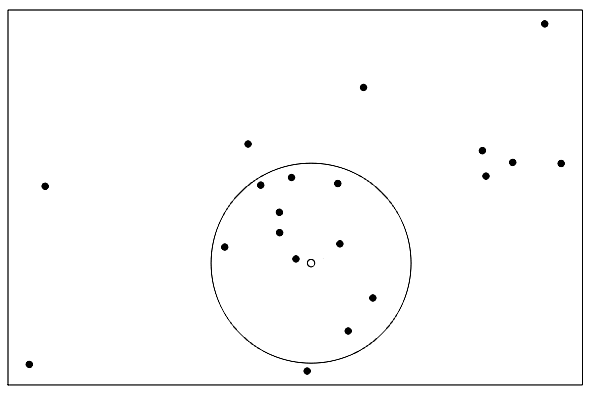
\includegraphics[width=.45\columnwidth]{gfx/ball_partition}} \quad
\subfloat[Generalised hyperplane Decomposition.] 
{\label{fig:hyperplane_decomposition}
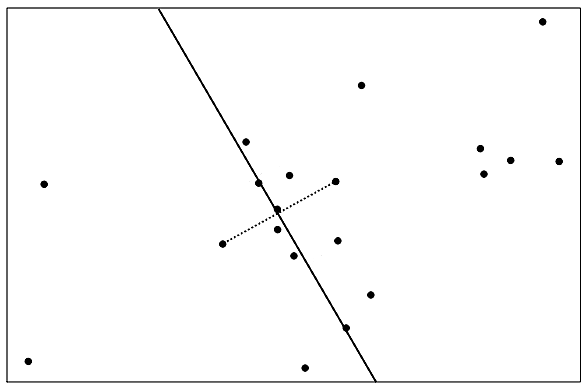
\includegraphics[width=.45\columnwidth]{gfx/hyperplane_partition}}
\caption[Ball Decomposition vs. Generalised hyperplane Decomposition]{Ball Decomposition -- the area inside the ball is one partition, the area outside is another.
Generalised hyperplane Decomposition -- those points nearest the first pivot form one partition, those nearest the other form another.}
\end{figure}
%
\subsubsection{Generalised hyperplane decomposition}
%
\begin{mydef}
Let $p_1$ and $p_2$ be two arbitary pivots selected from $S \subseteq X$.  Partition $S$ into two subsets $S_1$ and $S_2$ such that $S_1 = \{o_j : d(p_1, o_j) \leq d(p_2, o_j)\}$ and $S_2 = \{o_j : d(p_1, o_j) > d(p_2, o_j)\}$
\end{mydef}
% ********************** %
\subsection{Dimensionality}
% ********************** %
Bellman coined the term \textit{curse of dimensionality} referring to the exponential growth in the number of samples required to estimate a function with a given level of accuracy to its number of variables (or dimensions)\cite{Bellman:2003}.  This has a direct impact on similarity searching in that the number of points that must be visited to build the result of a query grows exponentially to the number of dimensions in the space.  In some cases, data may even be clustered together so tightly that the distance between the nearest neighbour and the farthest neighbour are the same, rendering any result meaningless.  In fact, it has been shown that these values converge as the number of dimensions increase%\cite{Indyk:1998}
%
\subsubsection{Measuring dimensionality}
Given the difficulty of indexing spaces with high dimensionality, a prudent approach would be to measure this. 
% [Here are the authors that have made a contribution, and what they have done]
%$d = \lim_{\epsilon \rightarrow 0} \frac{H_\epsilon(X)}{\log 1/\epsilon}$
%Intrinsic dimensionality
%
There is a great volume of work on the analysis of high-dimensional search spaces. Navarro gives a very elegant analysis of the history of this, along with some cogent insights into directions which could be usefully followed in the future, and bemoans the small volume of current research on the topic. 
%We follow his advice in that we attempt to find a general analysis rather than looking for reliance upon experiment or detailed analysis of particular data structures. Furthermore we also believe our analysis fulfils his longer-term goals of research in this domain which can underlie useful insight in the design of future techniques, rather than simply provide performance indicators.
%Other researchers also have advocated the analysis of performance based crucially upon the distribution of distances within the range of the metric over the objects of the space rather than on the data itself of the index structures, and we follow that lead.

%In \cite{}, a derivation for an exclusion probability e is given; this concept is technically equivalent to the probability pe we introduce in chapter \label{}, although we use a simplified version via the introduction of various assumptions. In spirit, this e is more similar to our IF , in that both are the probabilities of a pivoting operation failing to exclude some part of the data set from an exhaustive search.
%In the end, we deduce an outcome for the cost of a search in the order of (1 + IF ) ln n , rather than k + ne k , which is perhaps not inconsistent given that we use a much more restrictive indicative context.

%\subsection{Instrinsic Dimensionality}
%Our own work is more closely related to the description of Intrinsic Dimensionality as a performance predictor given in \cite{}. In particular it is applicable where the distance distribution strays from the ideal underlying Gaussian model, and where the fraction of data to be fetched is small.
%In common with \cite{}, the basis for measurement is only the set of distances produced by the metric with respect to the space, rather than the data itself, and our aim is to find a pragmatic measure of efficacy based only on the distribution of these distances. Both approaches allow for an automated assessment to be made only on presentation of a metric space with a random sampling mechanism.

The Intrinsic Dimensionality (IDIM) of a metric space is a measure defined over a distance histogram produced by the distance metric over the data. It is defined as
\[ 
\rho = \frac{\mu^2}{2\sigma^2}
\]
where $\mu$ is the expected distance and $\sigma^2$ is the variance of the range of the metric over the data collection. An IDIM of n corresponds roughly to the histogram of Euclidean distance over densely-populated n-dimensional Cartesian space. It is usually, but not always, the case that a higher value for IDIM leads to a worse performance of index structures for similarity search.

The authors give a lower bound for the cost of a pivoting operation as
\[ \left( \sqrt{\rho} - \frac{1}{\sqrt{2f}} \right)^2 \cdot \ln n\]
where $\rho$ is the IDIM, $f$ is the fraction of the data being returned, and $n$ is the size of the data. However this formula is valid only when $f > \frac{1}{2\rho}$, meaning that for large data sets, and therefore small values of $f$, it is of limited value.
The work uses an underlying assumption that the metric gives a Gaussian distribution of outcomes. 
%Figure 1 shows some distributions which are clearly not Gaussian; these are not artificially constructed, but show meaningful metrics in use over data sets within the SISAP collection [6].
More important, we believe, is that no metric distribution obeys a Gaussian distribution close to the origin as distances are by definition lower-bounded at zero, and we later show distributions very close to Gaussian where IDIM comparison is misleading as a predictor of performance.

In the discussion, the authors consider the same region of interest as here, the set of sampled distances which do not allow a median-centred pivot operation to successfully exclude any data from a search. 
%Our contributions over and above that are: (i) we note the fact that the distribution at the origin is crucially important in terms of selecting a value for the query threshold (t), and that the Gaussian model does not explain this; (ii) we note that the effect of t over the distribution is an effect of the standard deviation alone, and is unaffected by the value of the median, and (iii) by treating this region as a probability, by use of a probability density function rather than a histogram, we go on to calculate an actual indexing performance prediction based on a notional ball-pivot data structure.

%\subsubsection{Dimensionality reduction}
%Beyond simply measuring, some authors have approached the curse of dimensionality through a technique called dimensionality reduction. [Here are the authors that have made a contribution, and what they have done] 
%% *************** %
%\section{Summary}
%% *************** %
%In this chapter we have introduced the general concept of similarity search and justified its existence for types of data that do not lend themselves well to the existing methods of data storage.  We showed a useful mathematical abstraction called Metric Spaces, which allow us to reason about similarity in a way that produces efficient storage and retrieval.  Using the properties of Metric Spaces, we demonstrated the types of query that may be performed in such an abstraction, with emphasis placed on two in particular: range queries and nearest neighbour queries.  Next we quickly surveyed the principle metrics and data structures used in the storage and retrieval of data within the similarity search paradigm.  Finally we showed the limitations of using this abstraction, and in particular the curse of dimensionality with all of its negative implications.

% *************** %
\section{Probability \& Information Theory}
% *************** %
%\ToDo{Why are we looking at Probability?}
The frequentist view of probability is that there is a set of events that we assume occurs some number of times such that no two events can occur simultaneously. 
%
\begin{mydef}\label{prob}
let $E = \{ e_1, e_2, \ldots e_n \}$ be a sample space, some $F \subseteq E$ be an event space, and $P: E \rightarrow [0,1]$ a probability measure where $P$ satisfies the following axioms:
%
 \begin{align*}
  &P(F) \geq 0\\
  &P(E) = 1\\
  &P(\bigsqcup_{F \subseteq E} F) = \sum_{F \subseteq E} P(F)
 \end{align*}
%
\end{mydef} 
The probability must be positive, since a zero probability means it is certain not to happen you cannot be less certain of an event occurring than that.  The second axioms states that the probability that the next event occurring is from the set of all possible events is certain.  The third axiom states that the probability of an event occurring from the union of disjoint sets is the sum of probabilities from each of those disjoint sets. 
%
Furthermore the following derived properties also hold:
%
  \begin{align*}
  & P(\emptyset) = 0\\
  & P(F_1 \cup F_2) = P(F_1) + P(F_2) - P(F_1 \cap F_2)\\
  & P(E \setminus F) = 1 - P(F)
 \end{align*}
That is, the probability of an event occurring from the empty set is zero.  The probability of an event occurring from the union of two sets is the sum of  the probability of it coming from their respective sets minus the probability of the events that have been counted twice.  And the probability of an event occurring from outside a set is the probability of the sample space (which from the second axiom is 1) minus the probability of the event space.

A probability distribution assigns a probability to each subset.  
%Probabilities can be determined empirically as the number of times an event has occurred normalised by the total number of events.  
The proportion of times an event occurs relative to all events that have occurred is the probability of that event.

%\begin{myexample}
%Fair coin toss -- as is traditional when demonstrating probability.
%\end{myexample}
%
%\begin{myexample}
%Some other example
%\end{myexample}

% *************** %
\subsection{Information}
% *************** %
Suppose we have a probability function $P$, we can measure the information gained by observing an event based on the probability distribution of events.
%  
\begin{mydef}
Let $I: [0,1] \rightarrow \mathbb{R}$ be a monotonic function that measures the information gained by observing an event $e$ with probability $p = P(e)$, with the following axioms:
%
  \begin{align*}
  &\forall p, I(p) \geq 0\\
  & I(p) = 0 \Leftrightarrow p = 1\\
  & I(p_1 \cdot p_2) = I(p_1) + I(p_2)
  \end{align*} 
%
\end{mydef} 
%
The first axiom says that the information function must output a positive value;  it makes no sense to have lost information by witnessing an event.  The second says that there is no information to be gained by witnessing an event which we know is certain to occur.  The third says that the information gained after witnessing two events is the same as gaining the information from witnessing them separately.  A commonly used information function which obeys these axioms is $I(p) = -\log_b(p)$ for some base $b$.
%\begin{myexample}
%Some other example
%\end{myexample}
%\begin{myexample}
%Some other example
%\end{myexample} 
% *************** %
\subsection{Entropy}
% *************** %
%\ToDo{Why are we looking at Entropy?}
Given a stream of events whose probability is defined by the some function $P$ the average information gained per event is known as entropy.
%
\begin{mydef}
Let $S$ be some source emitting a stream of events from the set $E = \{e_1, e_2, \ldots, e_n\}$ with associated probabilities $P = \{p_1, p_2, \ldots, p_n\}$ respectively.

There are $N\cdot p_i$ occurrences of $e_i$ after $N$ observations, as $N$ approaches infinity.  So the total information gained is $I = \sum_{i = 1}^n (N \cdot p_i) \cdot I(p_i)$, and the average information per event is therefore:
\[ H(S) = \frac{I}{N} \]
Using $I(p_i) = -\log(p_i)$ gives,
\begin{align*}
H(S) &= \frac{1}{N} \cdot \sum_{i = 1}^n  (N \cdot p_i) \cdot -\log_b (p_i)\\
	 &= -\sum_{i = 1}^n  p_i \cdot \log_b (p_i)
\end{align*}  
\end{mydef}

%\begin{myexample}
%Some other example
%\end{myexample}
%\begin{myexample}
%Some other example
%\end{myexample}

\begin{mydef}
Let $S$ and $T$ be two sources emitting streams of events from the set $E = \{e_1, e_2, \ldots, e_n\}$.  Denote the probability of $S$ emitting $e_i$ and $T$ emitting $e_j$ as $p_{i,j}$.  Then the joint entropy of $S$ and $T$ is:
\[H(S, T) = -\sum_{i = 1}^n\sum_{j = 1}^n p_{i,j} \log_b (p_{i,j})\]
\end{mydef}

\subsection{Mutual Information}
\begin{mydef}
Let $S$ and $T$ be two sources emitting streams of events from the set $E = \{e_1, e_2, \ldots, e_n\}$. Then the mutual information between $S$ and $T$ is:
\[I(S,T) = H(S) + H(T) - H(S,T)\]
\end{mydef}

\subsection{Cross Entropy}
\begin{mydef}
Consider two sources, $S$ and $T$, emitting streams of events from the same set $E = \{e_1, e_2, \ldots, e_n\}$.  Let $S$ emit events with probability $P = \{p_1, p_2, \ldots, p_n\}$ and $T$ emit events with probability $Q = \{q_1, q_2, \ldots, q_n\}$.  If we model $S$ with $T$, $P$ is the true distribution and $Q$ is the model distribution. After $N$ observations, there are $N \cdot p_i$ occurrences of $e_i$, as $N$ approaches infinity, so the total information gained is $I = \sum_{i = 1}^n (N \cdot p_i) \cdot I(q_i)$, and the average information gained is:
\begin{align*}
H(S||T) 	&= \frac{I}{N}\\
	 	&= \frac{1}{N} \cdot \sum_{i = 1}^n  (N \cdot p_i) \cdot -\log_b (q_i)\\
	 	&= -\sum_{i = 1}^n  p_i \cdot \log_b (q_i)
\end{align*}  
\end{mydef}
This represents the average amount of surprise from observing an event when modelling a one distribution with another.
\subsection{Gibbs' inequality}
\begin{align*}
H(S||T) 	&\geq  H(S)\\
H(S||T) - H(S) &\geq 0\\
\end{align*}
The average amount of surprise when modelling one distribution with another is greater than if you had used the correct distribution.
\subsection{Relative Entropy}
This difference in entropies, $H(S||T) - H(S)$, is the relative entropy. Commonly known as K\"ullback-Liebler divegence; it is a measure of the divergence of information streams:
\begin{align*} 
KL(S||T)		&= H(S||T) - H(S)\\
			&= -\sum_{i = 1}^n  p_i \cdot \log_b (q_i) + \sum_{i = 1}^n  p_i \cdot \log_b (p_i)\\
			&= -\sum_{i = 1}^n  p_i \cdot (\log_b (q_i) - \log_b (p_i))\\
			&= -\sum_{i = 1}^n  p_i \cdot \log_b (\frac{q_i}{p_i})
\end{align*}
%The K\"ullback-Liebler divergence is derived directly from Shannon's original  definition of the entropy of a set of independent variables. Set in the context of a term-probability vector modelling a document $d$, the Shannon entropy is:
%%
%\[H_b(d) = - \sum_t \p(t|d) \log_b ( \p(t|d))\]

%In the context of the very sparse vectors used for the vector space model, it is worth explicitly noting that, for this purpose, the undefined term $0 \! \log(0)$ is normally taken as having a value of 0; this is reasonable as the term $\epsilon \log \epsilon \rightarrow 0$ as $\epsilon \rightarrow 0$.

%The meaning of the term $H_2(d)$ in our context is a theoretical lower bound for the mean number of bits%
%\footnote{From this point we will assume that all logs  are  base 2.}
% required to communicate each event in the stream generated by $\G^d$.

The information in event e for discrimination between distributions $P$ and $Q$, and the mean information for discrimination.
%For two generators $\G^v$ and $G^w$, then $KL(G^v,G^w)$ gives the extra  number of bits per event required to encode $G^w$ over $G^v$. This function is given by
%\[
%KL(v,w) = \sum_t  \p(t|v)  \log \! \left(\frac{\p(t|v)}{\p(t|w)}\right) 
%\]
As a general measure of difference, this function has a number of problems: it is asymmetric, unbounded, and undefined in the presence of zero values.

%The K\"ullback-Liebler divergence is derived directly from Shannon's original  definition of the entropy of a set of independent variables. For a  vector $v$ modelling a probability distribution, the Shannon entropy is:
%%
%\[H(v) = - \sum_{i} v_i \log ( v_i)\]

%In the context of the very sparse vectors used for the vector space model, it is worth explicitly noting that, for this purpose, the undefined term $0 \! \log(0)$ is normally taken as having a value of 0; this is reasonable as the term $\epsilon \log \epsilon \rightarrow 0$ as $\epsilon \rightarrow 0$.

%The meaning of the term $H(v)$ in our context is a theoretical lower bound for the mean number of bits%
%\footnote{if  base 2 logarithms are used}
% required to communicate each event in the stream of events corresponding to $v$.

%K\"ullback-Liebler is a measure of the divergence of information streams. For two probability vectors $v$ and $w$, then $KL(v,w)$ gives the extra  number of bits per event required to encode $w$ over the number required to encode  $v$. This function is given by
%\[
%KL(v,w) = \sum_i  v_i  \log \! \left(\frac{v_i}{w_i}\right) 
%\]
%As a general measure of vector difference, this function has a number of problems: it is asymmetric, unbounded, and undefined in the presence of zero values.

\subsection{Jensen-Shannon Divergence}
Lin \cite{Lin:1999}  further examined the $KL$ divergence and defined a modified function which shares the more desirable properties, and removes the undesirable ones.
\begin{mydef}
Consider two sources, $S$ and $T$, emitting streams of events from the same set $E = \{e_1, e_2, \ldots, e_n\}$.  Let $S$ emit events with probability $P = \{p_1, p_2, \ldots, p_n\}$ and $T$ emit events with probability $Q = \{q_1, q_2, \ldots, q_n\}$.  Consider a notional stream $U$ with probability distribution $R = \{r_1, r_2, \ldots, r_n\}$ for events in $E$ given by the function: 
\begin{equation*}
	P_R(e_i) = \frac{p_i + q_i}{2}
\end{equation*}

The Jensen-Shannon divergence is the average of the relative entropies, $KL(S||U)$ and $KL(T||U)$.
\begin{align*}
	JSD(S,T)		&= \frac{KL(S||U) + KL(T||U)}{2}\\
				&= \frac{-\sum_{i = 1}^n  p_i \cdot \log_b (\frac{r_i}{p_i}) -\sum_{i = 1}^n  q_i \cdot \log_b (\frac{r_i}{q_i})}{2}\\
				&= \frac{1}{2} \sum_{i = 1}^n	 p_i \cdot \log_b (\frac{p_i}{r_i}) + q_i \cdot \log_b (\frac{q_i}{r_i})
\end{align*}
\end{mydef}

%This function, generally known as Jensen-Shannon divergence, is given in its simplest form as
%\[
%JS(P,Q)  = KL(P,M) + KL(Q,M)
%\]
%where $M$ is the arithmetic  mean of $P$ and $Q$. 


%This function avoids the most problematic case, where the vectors $v$ and $w$ have a zero and a non-zero value respectively in the same dimension: as the vector $m$ is non-zero in that dimension, then  the $KL$ function is still well-defined%
%\footnote{division by zero is avoided but not $\log 0$; as both $\epsilon\log{\epsilon}$ and $\log \left(\frac{\epsilon}{\epsilon} \right)\cdot \epsilon \rightarrow 0$ as $\epsilon \rightarrow 0$ these terms are  taken as 0.}.

If base 2 logs are used, then the outcome is bounded in [0,1] with 0 meaning that the two distributions have equal probabilities for every event, and 2 meaning that for no event are both probabilities non-zero (see e.g. \cite{Lin:1999}). Despite being a simple derivation from K\"ullback-Liebler \cite{Lin:1999}, the Jensen-Shannon divergence is positive, symmetric, bounded and well-defined in all circumstances, and also has the identity property.

%There is a  form of Jensen-Shannon which is a proper distance metric. However, especially in the  context of sparse, high-dimensional vector spaces, even semantically close objects may have a significantly large threshold value. Intrinsic Dimensionality tends to be very high, even into the thousands; the combination makes the metric very poorly suited for metric search techniques.

Surprisingly recently, two authors \cite{endres:2003,OstVaj03} have independently established that the Jensen-Shannon divergence is the square of a proper metric. Since then, the metric has attracted some more interest in both statistics and information theory, and deeper analysis \cite{fuglede:paper} continues to show that the metric has some properties that, in short, should lend it to being, in many cases, the best possible semantic distance over any probabilistic generated form.
 
The fact that a form exists which is a proper metric immediately leads to the possibility of its use within metric indexing techniques. However any such excitement is short-lived in most cases; generative spaces are typically high-dimensional and sparse, and typical Intrinsic Dimensionality is very high -- possibly in the thousands -- excluding any possibility of successfully using metric indexing techniques.


%Kullback and Leibler describe the value $\log\frac{P_{x}(e)}{P_{y}(e)}$ as the information in event e for discrimination between distributions $x$ and $y$, and the mean information for discrimination -- nowadays known as the Kullback-Leibler divergence:
%\begin{align*}
%H(S) &= \frac{1}{N} \cdot \sum_{i = 1}^n  (N \cdot p_i) \cdot (\log_b (p_i) - \log_b(p_j))\\
%\end{align*} 
%
%
%\[
%KL(X,Y) = \sum_e P_{x}(e) \log\frac{P_{x}(e)}{P_{y}(e)}
%\]
%Jeffreys also used $\log\frac{P_{x}(e)}{P_{y}(e)}$ in %\cite{Jeffreys:1948} 
%but came up with a symmetrized version:
%\[
%J(X,Y) = \sum_e (P_{x}(e) - P_{y}(e)) \log\frac{P_{x}(e)}{P_{y}(e)}
%\]
%which turns out to have the value $KL(X,Y) + KL(Y,X)$.
%
%K\"ullback-Liebler divergence \cite{kullback_liebler} has been used to compare vector spaces in a number of different contexts. However it is of  limited use as a  general notion of dissimilarity: in particular, it is naturally asymmetric, unbounded, is not necessarily positive, and is undefined over any pair of distributions which contain zero probabilities. 

%Lin introduced the Jensen-Shannon divergence in \cite{Lin:1991} which is a symmetrized smoothed version of the Kullback-Leibler divergence:
%\begin{align}
%JSD(X,Y) &= \frac{KL(X,\frac{X+Y}{2}) + KL(Y,\frac{X+Y}{2})}{2}\notag\\
%&= \frac{\sum_e P_{x}(e) \log_2 \frac{P_{x}(e)}{P_{x \cup y}(e)} + \sum_e P_{y}(e) \log_2 \frac{P_{y}(e)}{P_{x \cup y}(e)}}{2}\notag\\
%&= \frac{1}{2}\sum_e P_{x}(e) \log_2 \frac{P_{x}(e)}{P_{x \cup y}(e)} + P_{y}(e) \log_2 \frac{P_{y}(e)}{P_{x \cup y}(e)}\label{eq:jsd}
%\end{align}


%Jensen-Shannon is the name commonly given to a divergence function first identified in \cite{Lin:1999}, in which some of the known deficiencies of the K\"ullback-Liebler divergence \cite{kullback_liebler} were investigated. We give a brief overview of the derivation.

%Lin \cite{Lin:1999}  further examined the $KL$ divergence  and defined a modified function which shares the more desirable properties, and removes the  undesirable ones. This function, generally known as Jensen-Shannon divergence, is given by
%\[
%JS(v,w)  = KL(v,m) + KL(w,m)
%\]
%where $m$ is the arithmetic  mean of $v$ and $w$. 

%This function avoids the most problematic case, where the vectors $v$ and $w$ have a zero and a non-zero value respectively in the same dimension: as the vector $m$ is non-zero in that dimension, then  the $KL$ function is still well-defined%
%\footnote{division by zero is avoided but not $\log 0$; as both $\epsilon\log{\epsilon}$ and $\log \left(\frac{\epsilon}{\epsilon} \right)\cdot \epsilon \rightarrow 0$ as $\epsilon \rightarrow 0$ these terms are  taken as 0.}.

%If base 2 logs are used and the result divided by two, then the outcome is bounded in [0,1] with 0 meaning that the two vectors have equal values in each dimension, and 1 meaning that for no dimension are both values non-zero \cite{Lin:1999}.
%% In this case, the function $D(v,w) = \sqrt{1 - JS(v,w)}$ is also a proper distance metric \cite{}.


% *************** %
\subsection{Kolmogorov Complexity}
% *************** %
Until now, we have discussed information in terms of random variables where entropy is average information.  Another approach instead  considers the actual information needed to specify strings of symbols.  The Kolmogorov complexity, $K(X)$, is the minimal length of any input which leads to the output $X$, for some fixed universal computer. The Kolmogorov complexity of the concatenation of two strings $X$ and $Y$, $K(XY)$, should be larger than $K(X)$ but cannot be larger than the sum $K(X)+K(Y)$
%\begin{quotation}\ToDo{paraphrase}
%In contrast to Shannon theory where the basic objects are random variables and entropies are average informations, algorithmic information theory deals with individual symbol strings and with the actual information needed to specify them. 
%To ``specify'' a sequence $X$ means here to give the necessary input to a universal computer $U$, such that $U$ prints $X$ on its output and stops. The analogon to entropy, called here usually the complexity $K(X)$ of $X$, is the minimal length of any input which leads to the output $X$, for fixed $U$. It depends on $U$, but it can be shown that this dependence is weak and can be neglected in the limit when $K(X)$ is large.
%
%Let us denote the concatenation of two strings $X$ and $Y$ as $XY$. Its complexity is $K(XY)$. It is intuitively clear that $K(XY)$ should be larger than $K(X)$ but cannot be larger than the sum $K(X)+K(Y)$. Even if $X$ and $Y$ are completely unrelated, so that one cannot learn anything about $Y$ by knowing $X$, $K(XY)$ is slightly smaller that $K(X) + K(Y)$. The reason is simply that the information needed to reconstruct $XY$ (which is measured by $K(XY)$) does not include the information about where $X$ ends and $Y$ starts (which is included of course in $K(X) + K(Y)$). The latter information increases logarithmically with the total length $N$ of the sequence $XY$. It is one of the sources for ubiquitous terms of order $\log(N)$ which become irrelevant in the limit $N \rightarrow \infty$, but make rigorous theorems in algorithmic information theory look unpleasant.
%\end{quotation}  